\documentclass[11pt,xcolor=svgnames]{beamer}
\usepackage{natbib,setspace}
\mode<presentation>

% replaces beamer foot with simple page number
\setbeamertemplate{navigation symbols}{}
%\setbeamerfont{frametitle}{series=\bfseries}
\setbeamercolor{frametitle}{fg=Black}

\setbeamertemplate{footline}{
   \raisebox{5pt}{\makebox[\paperwidth]{\hfill\makebox[20pt]{\color{gray}\scriptsize\insertframenumber}}}}

\graphicspath{{/green/Dropbox/inputs/},{/Users/mtaddy/Dropbox/inputs/}}

% colors
\newcommand{\theme}{\color{Maroon}}
\newcommand{\bk}{\color{black}}
\newcommand{\rd}{\color{DarkRed}}
\newcommand{\fg}{\color{ForestGreen}}
\newcommand{\bl}{\color{blue}}
\newcommand{\gr}{\color{black!50}}
\newcommand{\sg}{\color{DarkSlateGray}}
\newcommand{\nv}{\color{Navy}}
\setbeamercolor{itemize item}{fg=gray}

% common math markups
\newcommand{\bs}[1]{\boldsymbol{#1}}
\newcommand{\mc}[1]{\mathcal{#1}}
\newcommand{\mr}[1]{\mathrm{#1}}
\newcommand{\bm}[1]{\mathbf{#1}}
\newcommand{\indep}{\perp\!\!\!\perp}
\def\plus{\texttt{+}}
\def\minus{\texttt{-}}

% spacing and style shorthand
\setstretch{1.1}

\begin{document}

\setcounter{page}{0}
{ \usebackgroundtemplate{\includegraphics[height=\paperheight]{phoenix}}
\begin{frame}[plain]
\begin{center}

{\bf \LARGE \theme }

\vskip .25cm
{\bf \huge \theme Measuring Rhetoric \bk\vskip .2cm \Large Statistical Language Models in Social Science }

\vskip 1cm
Matt Taddy,  Chicago Booth


\vfill
{\texttt{faculty.chicagobooth.edu/matt.taddy/research}}

\end{center}
\end{frame} }

\begin{frame}
{History: \theme Text as data}

Social science text-as-data from the 1960s: \\~~~author identification in the Federalist papers.
\begin{center}
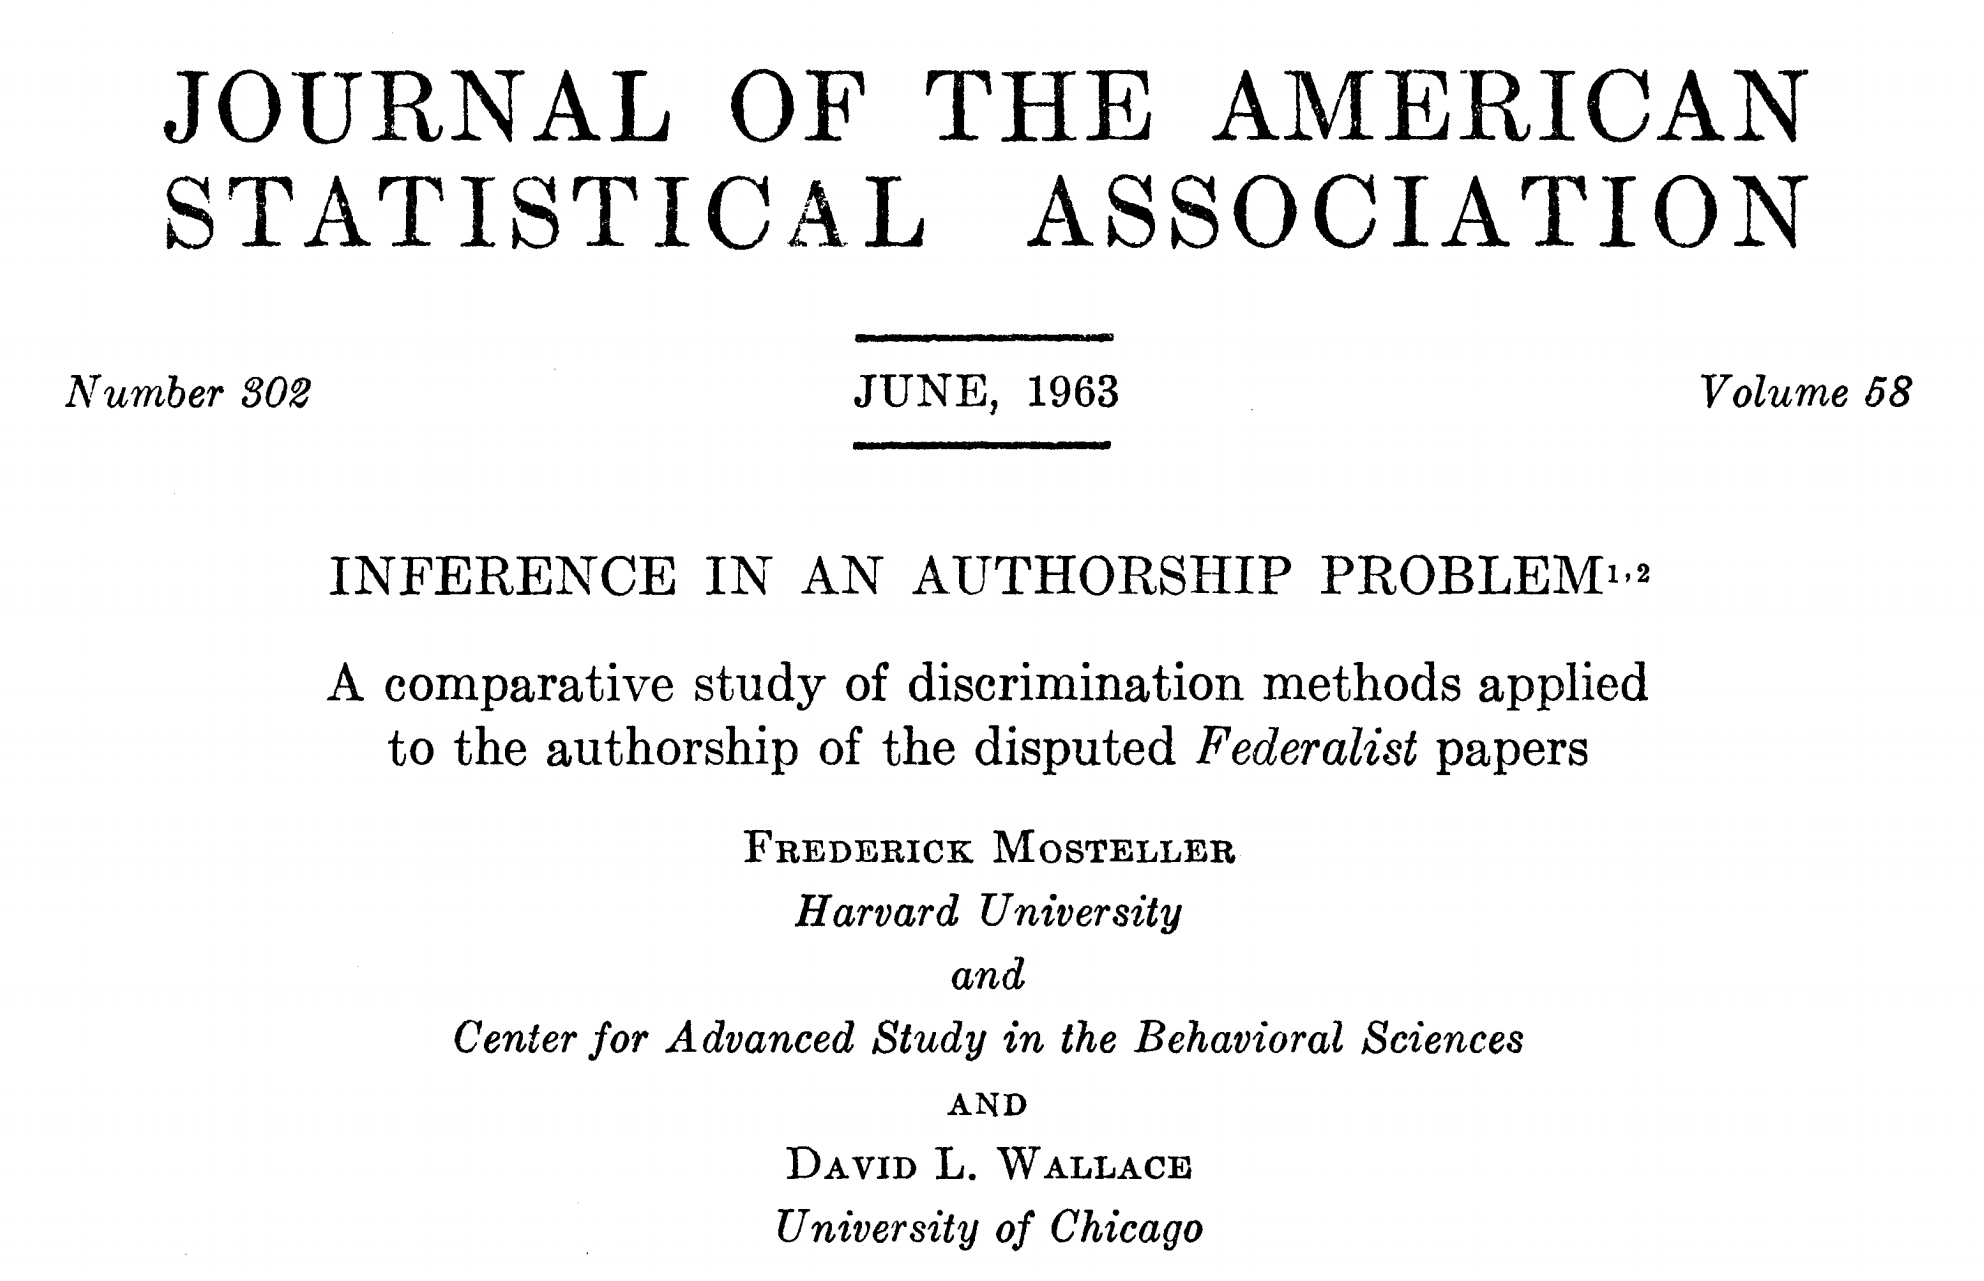
\includegraphics[width=3.75in]{../graphs/mostellerwallace}
\end{center}

\vskip -.5cm

\end{frame}

\begin{frame}
{History: \theme Text as data}


M{\tt+}W count words in papers by Hamilton and Madison,
\begin{center}
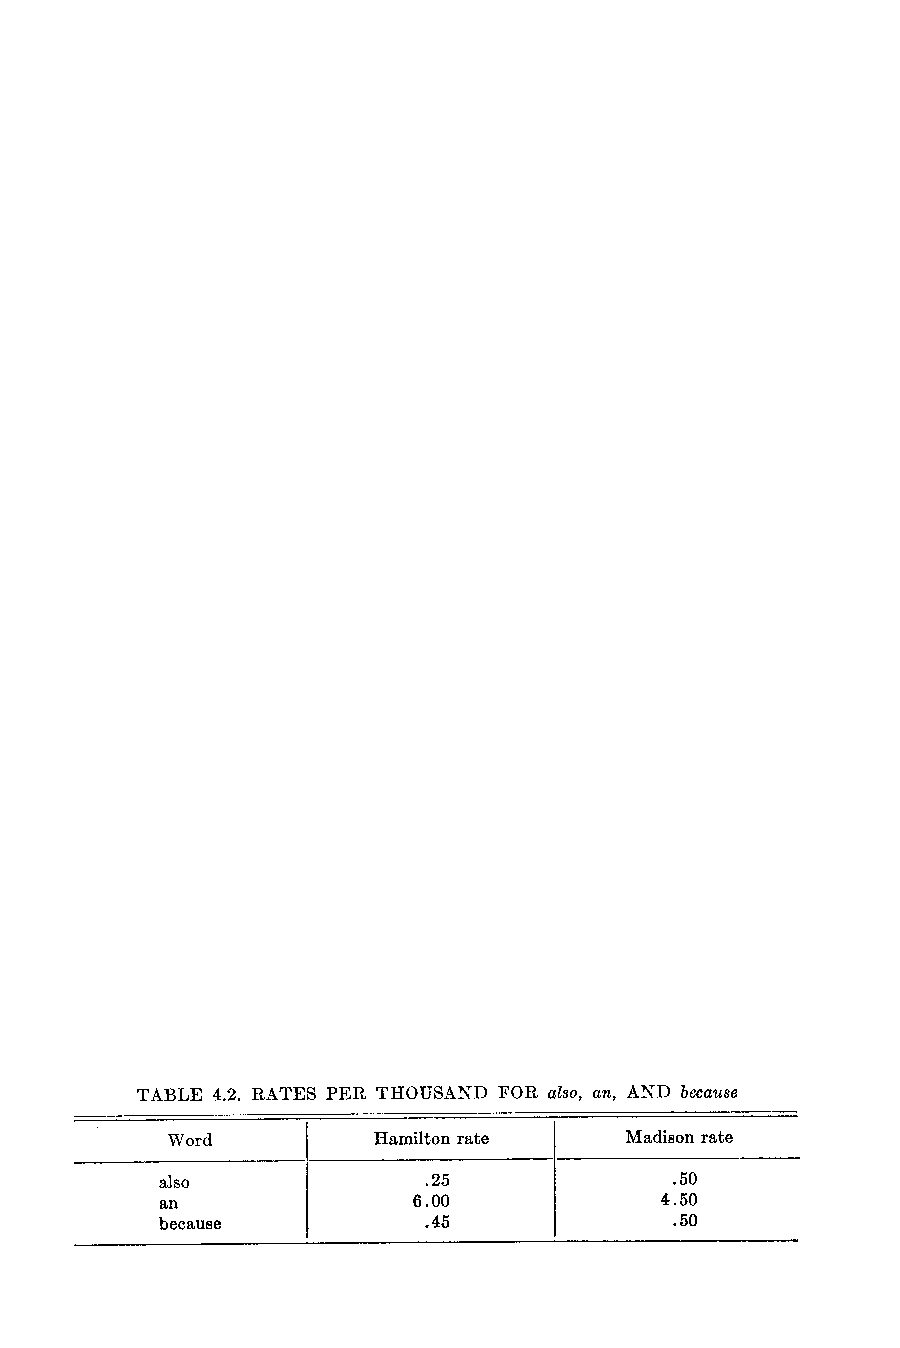
\includegraphics[width=4.25in]{../graphs/mostellertab}
\end{center}


then fit models for counts$|$author {\gr (essentially what I use today!)},
and use Bayes rule to predict authors$|$counts on disputed work.

{\large \nv\[\mr{p}(\text{Hamilton}\mid \text{text}) \approx 
\frac{\mr{p}(\text{text} \mid \text{Hamilton})}
{\mr{p}(\text{text} \mid \text{Madison}) + \mr{p}(\text{text} \mid \text{Hamilton})}
\]}

\end{frame}


\begin{frame}{
The `{\theme bag of words}'}

\vskip .25cm
 A `word' is a self-contained meaningful token...

\begin{itemize}
\item Actual words: `all', `world', `stage', `:-)', `{\tt \#textdata}'.
\item n-grams: `merely players' (bi), `men and women' (tri)
\item complicated clauses: parts of speech, act-of-god.
\item user selections on a website, domain ids in browser history 
\end{itemize}

All we do is count them.

\vskip .5cm

{\nv The remains state of the art!}

\vskip .1cm
Treat tokens for each doc as an i.i.d. sample. 

\vskip .1cm
Document $i$ is summarized by counts $c_{ij}$ for tokens $j=1...D$.

\vskip .1cm
Dumb but works: extra rules aren't worth their complexity.

\end{frame}

\begin{frame}
{Text as data \bk in Social Science}

\vskip .25cm
There's been an explosion of interest from social scientists.

 \vskip .25cm
Until very recently, one used pre-defined dictionaries.


\vskip .25cm
{Picking words: culturomics, Michel et al, Science 2011.}
\begin{center}
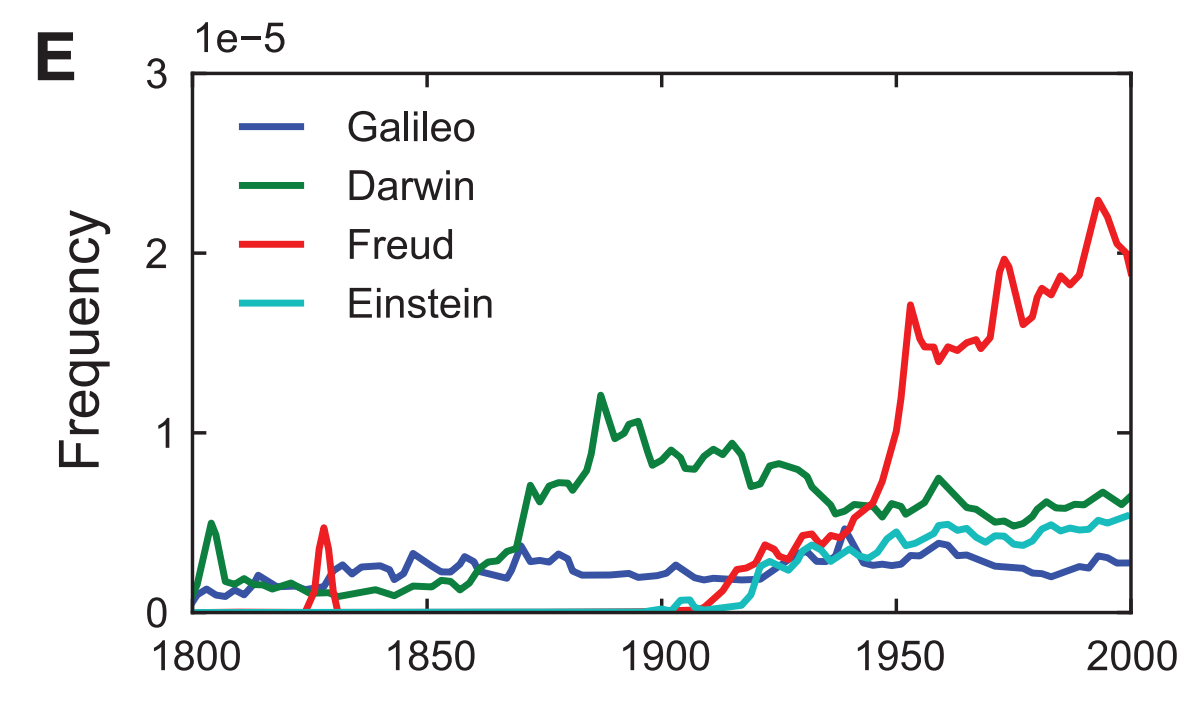
\includegraphics[width=2in]{../graphs/culturomics}
\end{center}


Psychosocial dictionaries, such as Harvard GI in {\it Tetlock 2007, Giving Content to Investor Sentiment} and others: 
\begin{center}
{\color{DarkGreen} able, abundant, accept} vs 
{\color{DarkRed} abandon, abrupt, absurd}.
\end{center}

\end{frame}

\begin{frame}
{Topic Models}

\vskip .25cm
Techniques from stats and ML are beginning to filter through and researchers are estimating relationships {\it from the data}.

\vskip .25cm  
A large area of research has developed around {\it topic models} 
\[\nv
\bm{c}_i \sim \text{MN}( \omega_{i1} \bs{\theta}_1 + \ldots + \omega_{iK} \bs{\theta}_K, m_i)
\]
{\it a multinomial with probabilities $\sum_k \omega_{ik}\bs{\theta}_{k}$ and total $m_i= \sum_jc_{ij}$.}

\vskip .5cm
This is a factor model for count data.

\vskip .1cm
Topics provide low-D structure, which the SS interprets.

{\gr Especially common in PoliSci; King, Grimmer, Quinn, ...}


\vskip .1cm
A big industry on extensions: dynamic TM, structural TM, ...

\end{frame}

\begin{frame}
{Topic Models Example}

\begin{center}
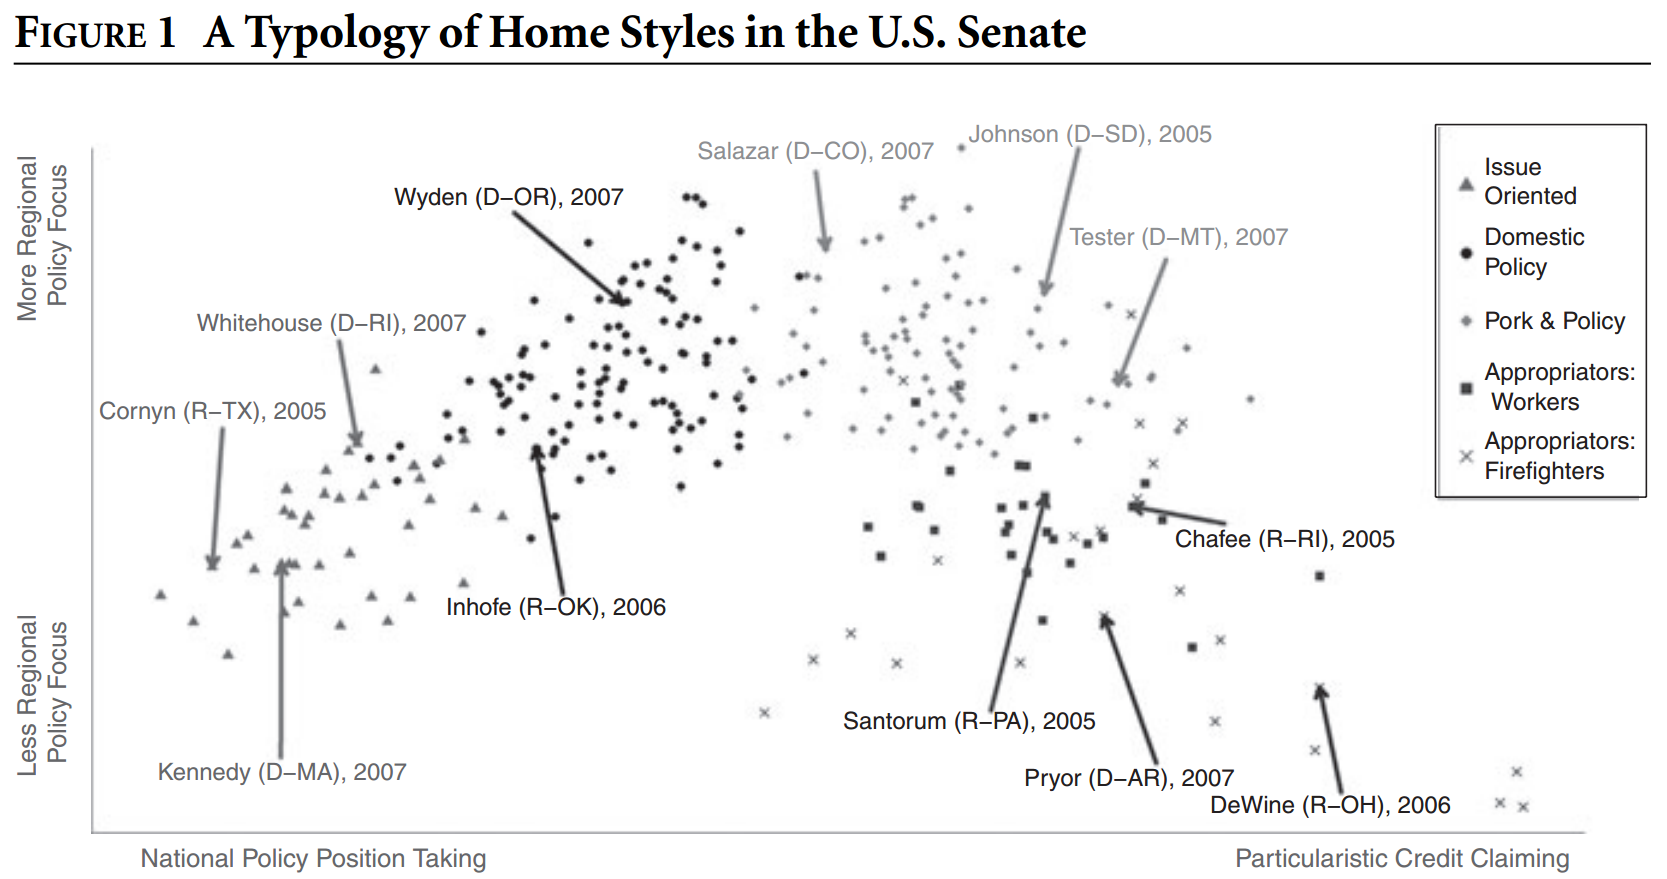
\includegraphics[width=3.75in]{../graphs/grimmer}
\end{center}


{\it Grimmer AJPS 2013:}  fit latent topics in press releases (e.g., `Iraq', `Infastructure') then investigate who uses what topic.

\end{frame}

\begin{frame}
{Multinomial Regression}

Instead of jumping straight to latent structure, perhaps we can answer our questions by regressing the text onto observables.


\vskip .5cm
Large response {\nv logistic regressions}: 

\vskip .2cm ~~~~$c_{ij}$ count for word $j$ in doc $i$, $m_i$ is total $\sum_j c_{ij}$

\vskip .2cm ~~~~$\bm{c}_i \sim \mr{MN}(\bm{q}_i, m_i)~~\text{with}~~
q_{ij} = e^{\eta_{ij}}/\sum_l e^{\eta_{il}}$

\vskip .2cm ~~~~${\nv  \eta_{ij} = \alpha_j + \bm{v}_i'\bs{\varphi}_{j}}$ is a `log intensity'  {\gr $\approx \mathrm{E}\log(c_{ij}/m_i)$}

\vskip .5cm
This is a regression like any other.   

\vskip .2cm
We will be estimating {\it partial correlations}, can build {\it random effects} and {\it interactions} into $\bm{v}$, ...  all our familiar regression ideas apply.

\end{frame}

\begin{frame}
{Distributed Multinomial Regression}

{\gr A regression like any other, except the response is super HD. }

We approximate the MN likelihood with {\it independent} Poissons: 
{\Large \nv \[
c_{ij} \sim \mr{Po}(~m_ie^{\eta_{ij}}~)
\]}
$\Rightarrow$ you can estimate each regression fully independently!

\vskip .5cm
This works because MN dependence is {\it only  induced by  totals}.

\vskip -.35cm
\[
\mr{MN}\left(\bm{c}_i;~\bs{\pi}_{i}/\Pi_i,
~m_i\right) = \frac{\prod_j
\mr{Po}\left(c_{ij};~\pi_{ij}\right)}
{\mr{Po}\left(m_i;~\Pi_i\right)}~~\text{where}~~\Pi_i = \sum_j \pi_{ij}
\]


DMR is equivalent to MN logit in a variety of simple examples,\\ and performs as well OOS in more complicated examples.
\vskip -.5cm

\end{frame}

\begin{frame}

answering social questions: yelp egs.

\end{frame}

\begin{frame}

Segregation in HD: adding random effects.  interpret SR as utility.

\end{frame}

\begin{frame}

moving to more complex language models: w2v and messaging.

\end{frame}

\end{document}
